

\begin{figure}[t]
    \subfloat[\integ\label{fig:result:overall:reproduction:integ}]{%
        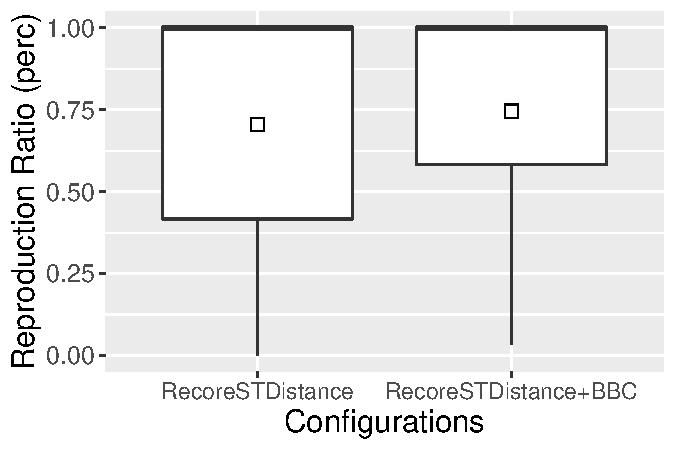
\includegraphics[width=0.45\textwidth]{papers/bbc/figures/reproduction-overall-recore.pdf}%
    }\hfil
    \subfloat[\WS\label{fig:result:overall:reproduction:ws}]{% 
        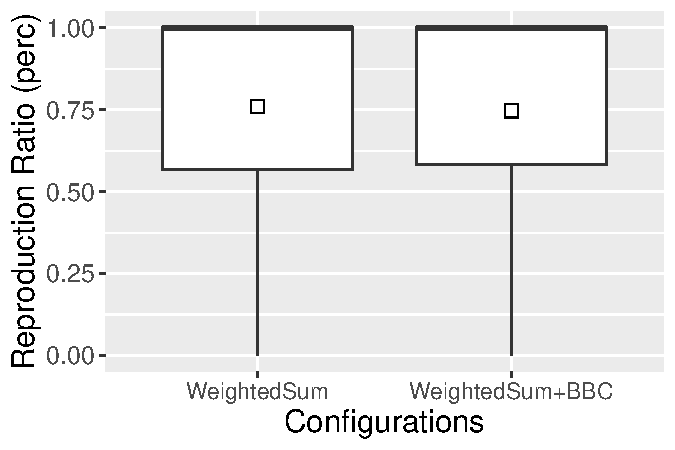
\includegraphics[width=0.45\textwidth]{papers/bbc/figures/reproduction-overall-ws.pdf}%
    }\hfil    
    \caption{Crash reproduction ratio (out of 30 executions) of fitness functions with and without \bbc. ($\square$) denotes the arithmetic mean and the bold line (---) is the median.}
    \label{fig:result:overall:reproduction}
\end{figure}

\begin{figure}[t]
    \subfloat[\integ\label{fig:result:significance:reproduction:integ}]{%
        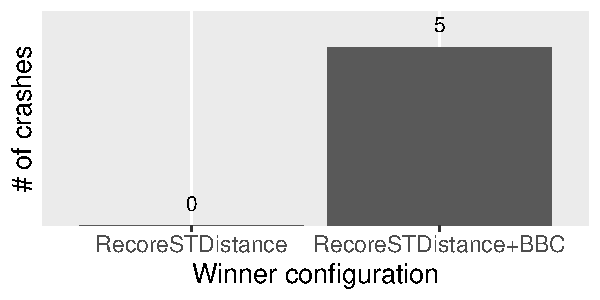
\includegraphics[width=0.45\textwidth]{papers/bbc/figures/significant-reproduction-recore.pdf}%
    }\hfil
    \subfloat[\WS\label{fig:result:significance:reproduction:ws}]{%
        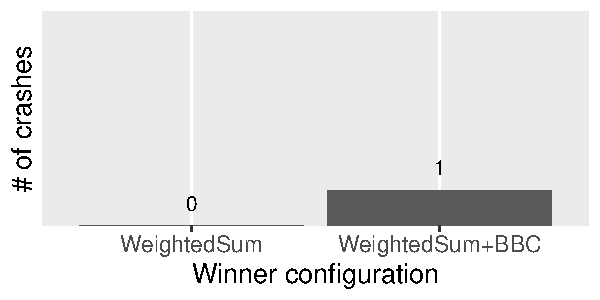
\includegraphics[width=0.45\textwidth]{papers/bbc/figures/significant-reproduction-ws.pdf}%
    }\hfil    
    \caption{Pairwise comparison of impact of \bbc on each fitness function in terms of crash reproduction ratio with a statistical significance $<0.01$.}
    \label{fig:result:significance:reproduction}
\end{figure}

\section{Results}
\label{sec:bbc:results}

\subsubsection{Crash reproduction effectiveness (RQ$_1$)}

Figure \ref{fig:result:overall:reproduction} presents the crash reproduction ratio of the search processes guided by \integ  (Figure \ref{fig:result:overall:reproduction:integ}) and \WS (Figure \ref{fig:result:overall:reproduction:ws}), with and without \bbc as a secondary objective. This figure shows that the crash reproduction ratio of \WS improves slightly when using \bbc. However, on average, the crash reproduction ratio achieved by \integ + \bbc is 4\% better than \integ without \bbc. Also, the lower quartile of crash reproduction ratio using \integ has been improved by about 30\% by utilizing \bbc.

Figure \ref{fig:result:significance:reproduction} depicts the number of crashes, for which \bbc has a significant impact on the effectiveness of crash reproduction guided by \integ (Figure \ref{fig:result:significance:reproduction:integ}) and \WS (Figure \ref{fig:result:significance:reproduction:ws}). 
\bbc significantly improves the crash reproduction ratio in 5 and 1 crashes for fitness functions \integ and \WS, respectively. Importantly, the application of this secondary objective does not have any significant negative effect on crash reproduction. Also, \bbc helps \integ and \WS to reproduce 6 and 1 new crashes, respectively (in at least one out of 30 runs), that could not be reproduced without \bbc.

\textbf{Summary. } \bbc slightly improves the crash reproduction ratio when using the \WS fitness function. However, on average, \bbc achieves a higher improvement when used as a secondary objective with the \integ function.

\begin{figure}[t]
    \subfloat[\integ\label{fig:result:significance:efficiency:integ}]{%
        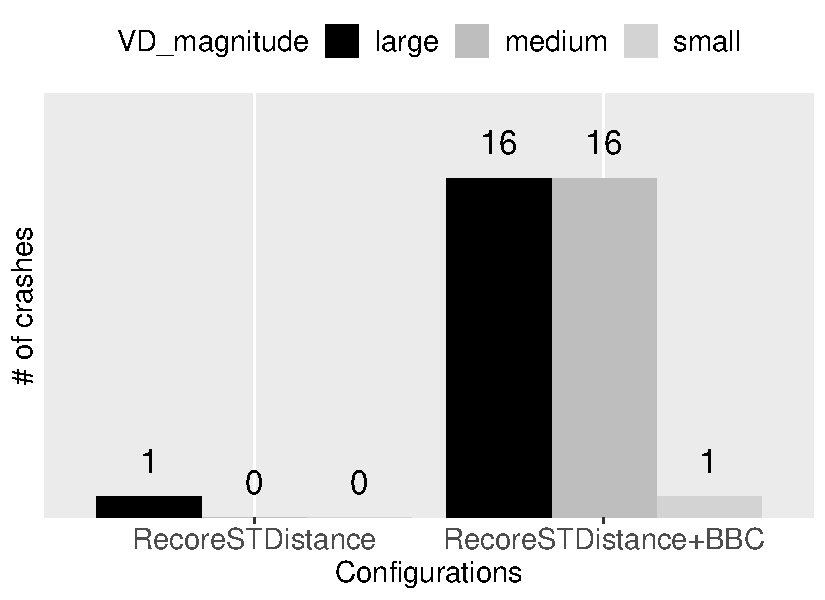
\includegraphics[width=0.45\textwidth]{papers/bbc/figures/significant-efficiency-recore.pdf}%
    }\hfil 
    \subfloat[\WS\label{fig:result:significance:efficiency:ws}]{%
        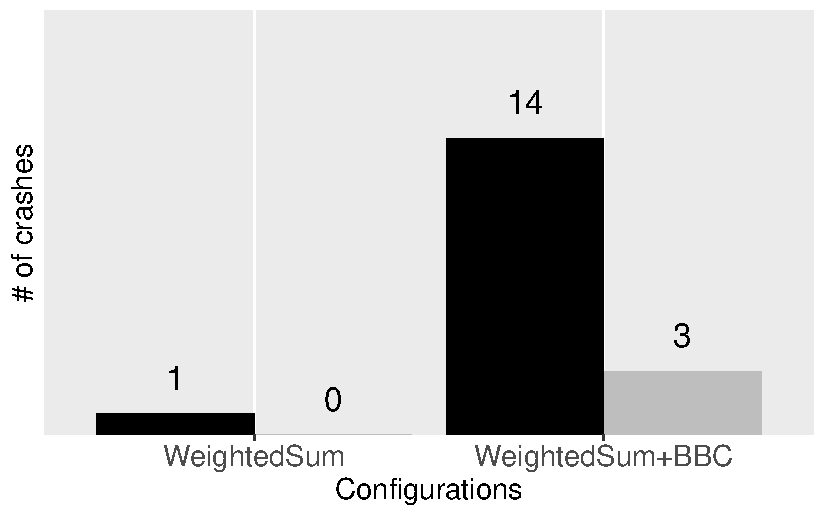
\includegraphics[width=0.45\textwidth]{papers/bbc/figures/significant-efficiency-ws.pdf}%
    }\hfil
    \caption{Pairwise comparison of impact of \bbc on each fitness function in terms of efficiency with a small, medium, and large effect size $\textit{\^{A}}_{12} < 0.5$ and a statistical significance $<0.01$.}
    \label{fig:result:significance:efficiency}
\end{figure}
\subsubsection{Crash reproduction efficiency (RQ$_2$)}

Figure \ref{fig:result:significance:efficiency} illustrates the number of crashes, in which \bbc significantly affects the time consumed by the crash reproduction search process. As Figure \ref{fig:result:significance:efficiency:ws} shows, \bbc significantly improves the speed of crash reproduction guided by \WS in 17 crashes (13.7\% of cases), while it lost efficiency in the reproduction of only one crash. In cases that \bbc significantly improves the efficiency of \WS, on average, the efficiency is improved for about 40\%.
Moreover,  Figure \ref{fig:result:significance:efficiency:integ} shows that \bbc has a higher positive impact on the efficiency of the search process guided by \integ. It significantly reduces the time consumed by the search process in 33 crashes (26.6\% of cases), while it had an adverse impact on the reproduction efficiency of only one crash. In cases that \bbc significantly improves the efficiency of \integ, on average, the efficiency is improved for about 53\%.

%Furthermore, Figure \ref{fig:result:improvement:efficiency} depicts the average improvement and the effect size of cases that \bbc had a significant impact on the efficiency of the search process. 
Figure \ref{fig:result:improvement:efficiency} depicts the average improvements in the efficiency and effect sizes for crashes where the difference in the consumed budget when using \bbc or not was significant.
According to the right-side plot in Figure \ref{fig:result:improvement:efficiency:integ}, \bbc reduces the time consumed by the search process guided by \integ up to 98\% (being 40.6\% on average).
Also, the left-side plot indicates that the average effect size of differences between \integ and \integ+\bbc (calculated by Vargha-Delaney) is~0.26 (lower than 0.5 indicates that \bbc improved the efficiency).
Figure \ref{fig:result:improvement:efficiency:ws} shows that the average improvement (right-side plot) achieved by using \bbc as the second objective of \WS is 44.3\%, and the average effect size (left-side plot), in terms of the crash reproduction efficiency, is 20.5.

\textbf{Summary. } \bbc improves the efficiency of the search process with both of the crash reproduction fitness functions.

\begin{figure}[t]
    \subfloat[\integ\label{fig:result:improvement:efficiency:integ}]{%
        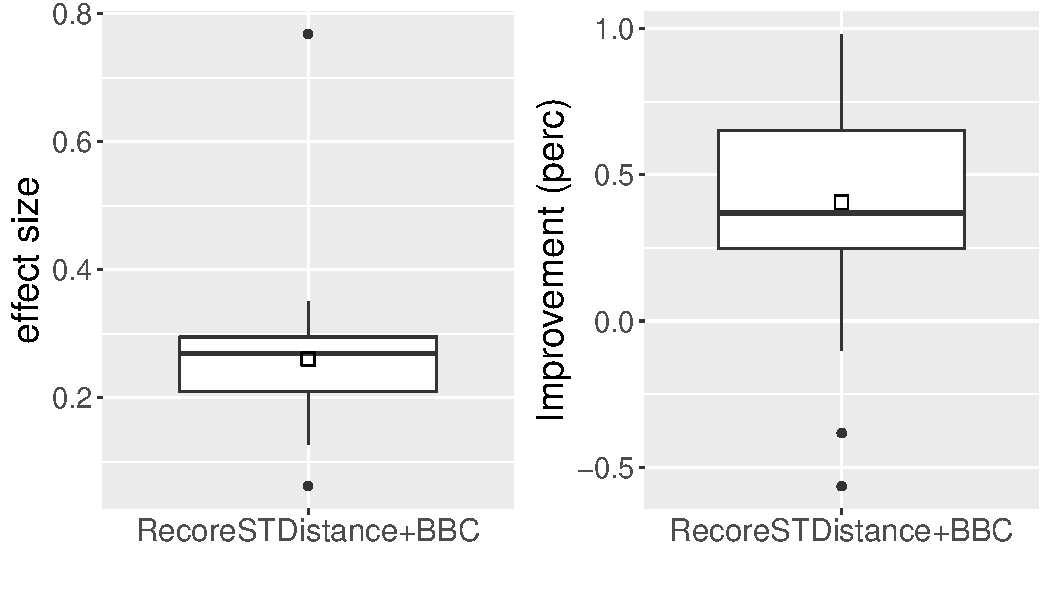
\includegraphics[width=0.5\textwidth]{papers/bbc/figures/improvement-efficiency-recore.pdf}%
    }\hfil 
    \subfloat[\WS\label{fig:result:improvement:efficiency:ws}]{%
        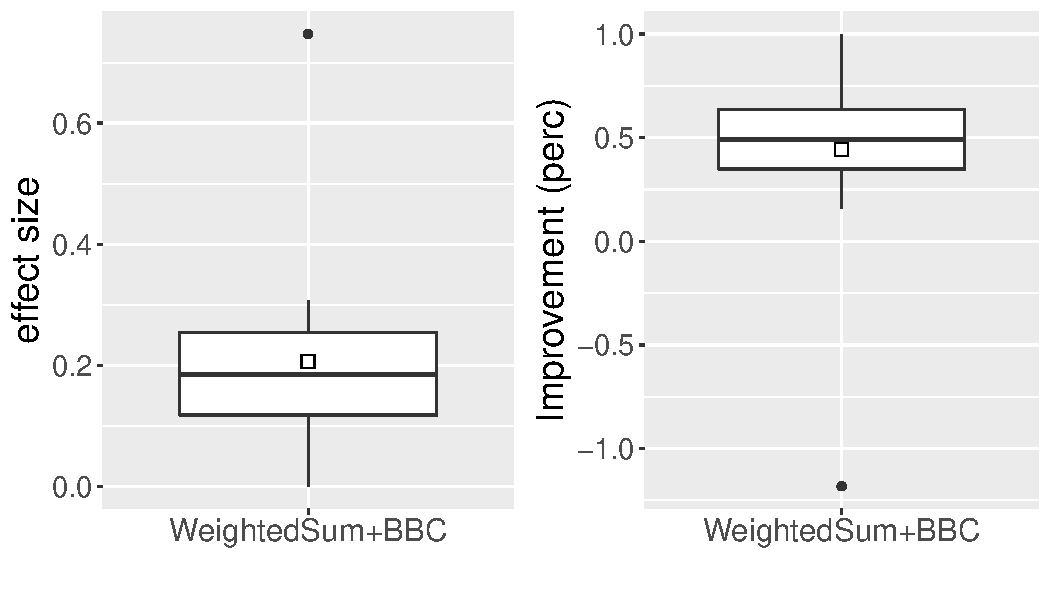
\includegraphics[width=0.5\textwidth]{papers/bbc/figures/improvement-efficiency-ws.pdf}% 
    }\hfil
    \caption{The effect size and the average improvement achieved by \bbc on each of the fitness functions in cases that \bbc makes a significant difference in terms of efficiency.}
    \label{fig:result:improvement:efficiency}
\end{figure} 



